% !TeX root = main.tex

%\setkeys{Gin}{draft}
\onehalfspacing
\section{Lab Assignment Goals}
\vspace{0.25cm}
\justifying 
This lab involved implementing a common source amplifier using the ALD1105 MOSFET to analyze the frequency response. The primary objectives included measuring the DC operating point, such as the drain current and voltage, and generating a Bode plot of the frequency response. Since the internal capacitances of the MOSFETs were too small for the laboratory equipment to measure, discrete capacitors were added to mimic their behavior. These measurements provided insight into optimizing amplifier performance for various applications. LTSpice was used to validate measurement techniques. 

\begin{center}
\begin{figure}[ht]
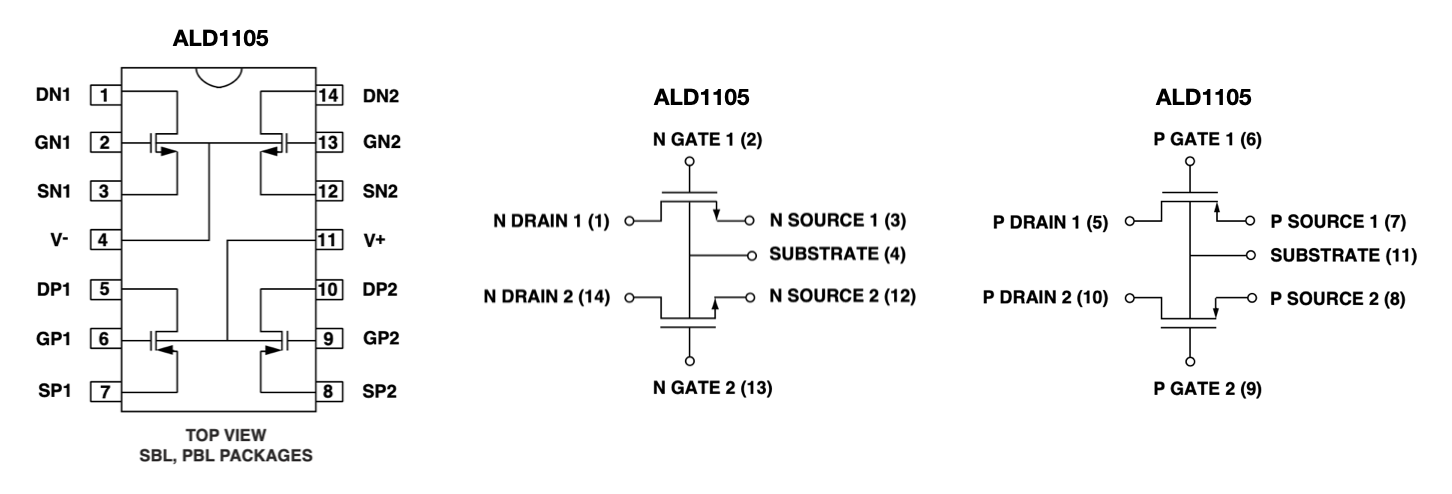
\includegraphics[scale=0.5]{Chapter_4/Lab_04_Image_1.png}
\caption{The pinout and block diagram of the ALD1105. \textbf{Note: $V^{-}$ is the body of the NMOS devices, which is connected to the lowest potential, and $V^{+}$ is the body of the PMOS devices, which is connected to the highest potential.}}
\label{Ch4_fig:1}
\end{figure}
\end{center}

\section{Experiment 1: DC Operating Point}

Using the circuit shown below with the given parameter values, the DC voltage $V_{GG}$ was adjusted such that the output voltage $V_{O}$ = $5$ V.

\begin{itemize}
    \item The DC operating point was determined by measuring the node voltages and calculating the currents. The summary table was then completed.
\end{itemize}

\begin{center}
\begin{circuitikz}[american]
\ctikzset{tripoles/mos style=arrows}
\draw

(-6,2) node[pmos,scale=2,xscale=-1] (Q3) {}
(4,2) node[pmos,scale=2] (Q2) {}
(4,-3) node[nmos,scale=2] (Q1) {}
(Q3.center) node[left] {$Q_{3}$}
(Q2.center) node[right] {$Q_{2}$}
(Q1.center) node[right] {$Q_{1}$}
(Q3.S) node[vdd] (vdd) {$+V_{DD}$}
(Q3.D) to[R=$R$] ++(0,-3) node[ground] {}
(Q3.D) to[short,*-] ++(2.5,0) to[short,-*] ++(0,1.53)
(Q3.G) -- (Q2.G)
(Q3.G) to[open,-*] ++(3,0) to[C=$C_{5}$] ++(0,2) node[ground,rotate=180] {}
(Q2.S) node[vdd] (vdd) {$+V_{DD}$}
(Q1.S) node[ground] {}
(Q2.D) -- (Q1.D)
(Q1.G)  to[short] ++(-2,0) to[C=$C_{B}$] ++(-2,0) to[R=$R_{sig}$] ++(-2,0) to[vsource,l=$v_{sig}$] ++(0,-3) node[ground] {}
(Q1.G) to[short] ++(-1.5,0) to[R=$R_{G}$,*-] ++(0,2) node[vdd] (vdd) {$+V_{G}$}
(Q1.G) to[short] ++(-1.5,0) to[C=$C_{1}$] ++(0,-2) node[ground] {}
(Q1.G) to[short] ++(-0.5,0) to[short,*-] ++(0,1.5) to[C,l=$C_{2}$,-*] ++(2.45,0)
(Q2.G) to[short] ++(-0.5,0) to[short,*-] ++(0,-1.5) to[C,l_=$C_{4}$,-*] ++(2.45,0)
(Q1.D) to[open] ++(0,1) node[left] {$V_{O}$}
(Q1.D) to[open] ++(0,1) to[C=$C_{B}$,*-] ++(3,0) to[R=$R_{L}$,v=$v_{o}$,*-] ++(0,-3) node[ground] {}
(Q1.D) to[open] ++(0,1) to[open] ++(3,0) to[short] ++(2,0) to[C=$C_{3}$] ++(0,-3) node[ground] {}
;
\end{circuitikz}
\end{center}

\section{Experiment 2: Frequency Response}

By employing appropriate AC measurement techniques, the frequency response of the amplifier was determined. The frequency range analyzed spanned from 10 Hz to 100 kHz. The following tasks were completed:

\begin{itemize}
    \item The mid-band gain $\left|G_{v\text{(mid)}}\right|$ was found.
    \item The bandwidth was determined by measuring $f_{L}$ and $f_{H}$, followed by computing the Gain Bandwidth Product (GBW) in Hz. The mid-band gain was converted to V/V.
    \item The measured and simulated results were plotted on the same curve, ensuring a magnitude range of 0 to +30 dB.
    \item The results for each experiment have been provided in the following tables.
    \item Calculations were done using Python and Simulations ran using LTSpice.
\end{itemize}

\newpage



\begin{center}

\begin{table}[H]
\begin{tabular}{ | >{\centering\arraybackslash} m{2.5cm} | >{\centering\arraybackslash} m{2.5cm} |  >{\centering\arraybackslash} m{2.5cm} | >{\centering\arraybackslash} m{2.5cm} | >{\centering\arraybackslash} m{2.5cm} |}
\hline
\multicolumn{5}{|c|}{DC Operating Point}        \\ \hline
                 Device & Quantity & Simulated  & Measured & Units \\ \hline
\multirow{5}{*}{$Q_{1}$} & $I_{D}$  & -485.30 & -492.70 & $\mu$A   \\ \cline{2-5} 
                  & $|V_{OV}|$ & 1.25 & 1.30 & V \\ \cline{2-5} 
                  &  $V_{G}$ & 1.85 & 1.85 & V  \\ \cline{2-5} 
                  & $V_{D}$ & 5.10 & 4.967 & V \\ \cline{2-5} 
                  & $V_{S}$ & 0.00 & 0.05 & V \\ \hline
                  &  &  &  &  \\ \hline
\multirow{5}{*}{$Q_{2}$} & $I_{D}$  & -473.564 & -492.70 & $\mu$A   \\ \cline{2-5} 
                  & $|V_{OV}|$ & 2.250 & 2.224 & V \\ \cline{2-5} 
                  &  $V_{G}$ & 7.103 & 7.129 & V  \\ \cline{2-5} 
                  & $V_{D}$ & 5.058 & 4.980 & V \\ \cline{2-5} 
                  & $V_{S}$ & 10.000 & 10.000 & V \\ \hline
                  &  &  &  &  \\ \hline
\multirow{5}{*}{$Q_{3}$} & $I_{D}$  & -473.564 & -473.600 & $\mu$A   \\ \cline{2-5} 
                  & $|V_{OV}|$ & 2.221 & 2.250 & V \\ \cline{2-5} 
                  &  $V_{G}$ & 7.120 & 7.100 & V  \\ \cline{2-5} 
                  & $V_{D}$ & 7.120 & 7.100 & V \\ \cline{2-5} 
                  & $V_{S}$ & 10.000 & 10.000 & V \\ \hline
\end{tabular}
\caption{DC Summary Table}
\end{table}

\begin{table}[H]
\begin{tabular}{ | >{\centering\arraybackslash} m{3.5cm} |  >{\centering\arraybackslash} m{3cm} | >{\centering\arraybackslash} m{3cm} | >{\centering\arraybackslash} m{2cm} |}
\hline
\multicolumn{4}{|c|}{AC Summary}        \\ \hline
                 Quantity & Simulated  & Measured & Units \\ \hline
$\left|G_{v\text{(mid)}}\right|$  & 27.325  & 17.361  & V/V   \\ \cline{1-4} 
$\left|G_{v\text{(mid)}}\right|$ & 28.731  & 24.791  & dB \\ \cline{1-4} \hline
 &  &  &  \\ \hline
$f_{L}$  & 44.668  & 101.604  & Hz   \\ \cline{1-4}
$f_{H}$ & 13.490  & 3.937  & kHz \\ \cline{1-4} \hline
 &  &  &  \\ \hline
$BW$  & 13.445  & 3.835  & kHz   \\ \cline{1-4}
$GBP$ & 367.384  & 66.582  & kHz \\ \cline{1-4} \hline
\end{tabular}
\caption{AC Summary Table}
\end{table}

\end{center}

%\clearpage
%\newpage

\section{Python Code Listings}

The Python implementation for frequency response analysis can be found in the Appendix (\cref{lst:Ch4:List1}).

\section{Conclusion}
\onecolumn
\justifying
\par
This lab focused on analyzing the frequency response of a common source amplifier by measuring its DC operating point, generating a Bode plot, and comparing simulated and measured data. Python code for this lab can be foud in the code listing \cref{Ch4:List1}. The process included adjusting the biasing conditions, sweeping the frequency response, and capturing key characteristics such as the lower and upper cutoff frequencies ($f_L$ and $f_H$), gain bandwidth product (GBP), and mid-band gain ($G_v$). The measured high-frequency cutoff ($f_H$) was found to be lower than the simulated value, indicating additional parasitic effects or variations in component behavior. The Miller Effect causes large discrepacies in the values between simulated and measured. The Miller effect states that if an impedance ($Z$) is in parallel with an inverting amplifier with a gain of magnitude $A$ (Figure 3, left), it can be split into two separate impedances at the input and output of the amplifier (Figure 3, right). 
The input and output impedances have values of $Z_{in} = \frac{1}{Z_1 + \frac{1}{A}}$ and $Z_{out} = \frac{Z_1}{1+A}$, respectively, and are both tied to ground.
\vspace*{0.10cm}
\par
Another critical factor is the \textbf{Miller effect}, which significantly impacts the high-frequency response of the amplifier. The Miller effect describes how the capacitance between the drain and gate ($C_{gd}$) is amplified by the voltage gain of the stage, effectively increasing the equivalent input capacitance. This phenomenon lowers the bandwidth by reducing the effective high-frequency cutoff. In simulations, SPICE models may not fully capture all secondary Miller capacitance effects, especially if they do not account for layout-dependent parasitics. In practical circuits, additional unintended capacitances and PCB trace effects further exacerbate the Miller effect, further decreasing the measured $f_H$ compared to the simulated value.
\vspace*{0.10cm}
\par
Results demonstrated how real-world variations influence circuit performance and emphasized the importance of simulation validation. Future work may involve refining the biasing network and improving frequency response accuracy through component selection and layout optimization.
